\section{Using a Virtual Machine}

Just like a tree-walking interpreter, a virtual machine presents a way of implementing an interpreter for a programming language.
However, the way a virtual machine operates differs fundamentally from a tree-walking interpreter.
In order to compare the two, we have implemented a virtual machine backend for rush.

\subsection{Defining a Virtual Machine}

Often, one might encounter the term \emph{virtual machine} (\emph{VM}) when talking about emulating an existing type of computer using a software system.
This emulation typically includes additional devices like the computer's display or its disk,
whereas in this context, the term only describes a software entity which emulates how a processor interprets instructions.
Since the VM is unable to traverse the AST, it depends on a compiler generating its input instructions.

Because a physical processor and a virtual machine share some fundamental traits,
the architecture of a virtual machine is often closely resembling the \emph{von Neumann architecture}.
This architecture was first introduced by John Neumann in the year 1945.
Von Neumann originally presented a design which allows implementing a computer using relatively few components.
Following the von Neumann architecture, a processor would usually contain components like an \emph{arithmetic logic unit} (\emph{ALU}), a control unit, multiple registers, memory, and basic IO~\cite[p.~172]{Ledin2020-yp}.
The ALU's task is to perform logical and mathematical operations.
Which ones is being told by the control unit within the \emph{fetch-decode-execute} cycle.
This cycle is a simplification of the steps a processor performs in order to execute instructions.
The list below explains its individual steps~\cite[pp.~208--209]{Ledin2020-yp}.

\begin{itemize}
	\item \textbf{Fetch}: The processor's control unit loads the next instruction from the adequate memory location.
	      The instruction is then placed into the processor's internal instruction register where it is available for further analysis.
	\item \textbf{Decode}:
	      The processor's control unit examines the fetched instruction in order to determine whether additional steps must be taken before or after instruction execution.
	      Such steps may involve accessing additional registers or memory locations.
	\item \textbf{Execute}:
	      The control unit dispatches the instruction to a specialized component of the processor.
	      The target component is often dependent on the type of instruction since each processor component is designed with one specific type in mind.
	      For instance, the control unit may invoke the ALU to execute a mathematical instruction.
\end{itemize}

A computer's processor performs this fetch-decode-execute cycle repeatedly from the moment it powers on to the point in time when it shuts down again.
For relatively simple processors, each cycle is executed in isolation because instructions are executed in a sequential order.
This means that the execution of the instruction $i$ is delayed until execution of $i - 1$ has completed~\cite[pp.~208--209]{Ledin2020-yp}.
More sophisticated processors often use many performance-enhancing techniques like \emph{SIMD processing} or \emph{simultanious multithreading}~\cite[pp.~217f]{Ledin2020-yp}.

In most cases, a virtual machine executes instructions similarly to the fetch-decode-execute cycle.
Although the von Neumann architecture is relatively simple, one does not always have to adopt it when implementing a virtual machine.
Since virtual machines are purely abstract constructs without physical limitations, design constraints are usually kept to a minimum.
Therefore, a virtual machine can also be implemented with the high-level abstractions of its input language in mind.
For instance, the VM might feature specialized `break', `continue', or `loop' instructions which are not present in modern-day CPUs.
Designing the architecture of a virtual machine can sometimes be a challenging task since choosing an adequate set of features may involve a lot of testing iterations.
Because neither the compiler nor the VM exist in the beginning, one should carefully plan the implementation of their VM's architecture.

\subsection{Register-Based and Stack-Based Machines}

One of the main decisions to be made during the design of the VM is how it implements temporary storage.
Physical processors often use \emph{registers} in order to make larger computations feasible.
Registers are a limited set of very fast, low capacity storage units.
On most relevant architectures today, like \emph{x86\_64}, each general-purpose register is able to hold as much as 64 bits of information.
However, there is always only a limited amount of registers available since they are physical components of the CPU\@.
Therefore, programs typically only utilize registers for storing temporary values, such as intermediate results of a large computation.
The main alternative to registers is a stack-based design.
A popular example for a stack-based virtual machine is \emph{WebAssembly}~\cite[p.~44]{Sendil2022-fy}.
For more information on WebAssembly, Section~\ref{sec:wasm} presents a compiler targeting it.
For compiler writers, managing registers is often a demanding task.
This problem is described thoroughly in Chapter~\ref{chap:low_level_targets}.
On the other hand, targeting stack-based machines is usually significantly easier compared to register-based ones.
Therefore, one might choose to implement a stack-based virtual machine in order to minimize the complexity of both the compiler and the interpreter.
However, a stack-based design also introduces several issues on its own.
For example, register-based machines might regularly outperform stack-based machines.
A possible reason for this is that utilizing the stack typically requires a lot of seemingly redundant push and pop operations.

\subsection{The rush Virtual Machine}

The rush virtual machine is a stack-based machine implemented using the Rust programming language.
The machine's architecture was solely developed for this project and includes a \emph{stack} for storing short-term data, \emph{linear memory} for storing variables, and another separate \emph{call stack} for managing function calls.
Like most virtual machines, the rush VM uses a fetch-decode-execute cycle in order to interpret programs.

\Lirsting[ranges={16-26}, caption={Struct definition of the VM.}, label={lst:vm_struct}, float=h]{deps/rush/crates/rush-interpreter-vm/src/vm.rs}

Listing~\ref{lst:vm_struct} displays the struct definition of the rush VM\@.
The \qVerb{stack} field in line~18 saves the main stack for temporary values.
In line~20, the \qVerb{mem} field is declared.
This field represents the linear memory used for storing variables.
Since the \qVerb{Value} is wrapped in an \qVerb{Option}, each cell may also hold a \qVerb{None} value representing uninitialized memory.
In line~23, the \qVerb{mem_ptr} field is declared.
It holds the \emph{memory pointer}, which saves the index of the last free cell in \qVerb{mem}.
Lastly, a field named \qVerb{call_stack} is declared.
This field is responsible for managing function calls and returns.

The instructions in Listing~\ref{lst:tree_vs_vm_vm} on page~\pageref{lst:tree_vs_vm_vm} can be interpreted by the rush VM\@.
Programs for the rush VM are always partitioned into functions which each represents a sequence of instructions.
Since function and variable names are replaced by indices, human-readable names causing inefficiencies can be omitted entirely.
For better understanding, the individual functions have been manually annotated with their human-readable names.

\begin{wrapfigure}{L}{0.54\textwidth}
	\begin{NiceTabular}{>{\scriptsize}c}[name=Left]
		\\
		\\
		\\
		\Verb{num}       \\
		\Block[draw]{} 9 \\
	\end{NiceTabular}\hspace{1cm}
	\begin{NiceTabular}
		[
			first-col,
			%code-for-first-col=\ValueMinusOne{iRow},
			first-row,
			hvlines,
			colortbl-like,
			name = Right
		]
		{cc>{\scriptsize}c}
		 & Cell                  & $rel$  & {\normalsize abs} \\
		 & a                     & $-3$   & $mp + rel = 0$    \\
		 & b                     & $-2$   & $mp + (-2) = 1$   \\
		 & c                     & $-1$   & $mp - 1 = 2$      \\
		 & d                     & $0$    & $mp = 3$          \\
		 & \cellcolor{gray!30} e & $1$    & $mp + 1 = 4$      \\
		 & \ldots                & \ldots & \ldots            \\
	\end{NiceTabular}

	\begin{tikzpicture}[overlay,remember picture]
		\draw [->] (Left-5.5-|Left-last) to [bend left] (Right-5.5-|Right-1);
		\draw [thick, dashed] (Right-4.5-|Right-5) --  node[anchor=west, xshift=-1cm, align=center] {\scriptsize memory\\ \scriptsize pointer $= 3$} ([xshift=2.5cm]Right-4.5-|Right-4);
	\end{tikzpicture}
	\caption{Linear memory of the rush VM.}\label{fig:rush_vm_linmem}
\end{wrapfigure}

The first block of instructions is called \emph{prelude}.
Its only task is to declare global variables and call the `\texttt{main}' function.
Global variables need to be initialized at the beginning of a program so that they can be accessed later.
If the prelude was omitted, the \qVerb{main} function would instead have to contain these instructions since it is executed at program start.
However, recursion of the \qVerb{main} function is allowed in rush.
Therefore, each time the \qVerb{main} function recurses, all global variables would be restored to their initial values.
In order to prevent this bug, the rush VM uses a prelude function which is guaranteed to only run once.

Linear memory in the VM is represented as an array of runtime values of variables.
Each storage cell can be accessed through two different addressing modes.
When using the \emph{absolute addressing} mode, the exact index of the memory cell is specified.
For instance, if the value of the variable \qVerb{num} in Figure~\ref{fig:rush_vm_linmem} was to be retrieved,
the VM would need to access the storage cell with the absolute index `4'.
However, the absolute position of a variable in memory can only be determined at runtime.
For example, in a recursive function, each recursion adds another scope containing variables, thus allocating more memory.
However, the rush VM also implements a \emph{relative addressing} mode which can be used without knowledge about the absolute position of the memory cell.
For instance, the same variable can also be addressed through index `1' using the relative addressing mode.
The mode is called \emph{relative} because all addresses are specified relative to the memory pointer.
In Figure~\ref{fig:rush_vm_linmem}, the memory pointer (shortened to $mp$) is set to `3'.
Considering the value of the memory pointer, the absolute address of any relative address can be calculated at runtime.
Here, the absolute address is the sum of the relative index $rel$ and the runtime memory pointer $mp$.
By also implementing this relative addressing mode,
compilers targeting the rush VM can generate code without knowing the runtime behavior of a program.
For better understanding, Figure~\ref{fig:rush_vm_linmem} can be considered more closely.
Here, the first column contains a character to identify each memory cell.
The second column specifies the relative address of the cell, assuming that $mp$ is set to `3'.
Lastly, the third column contains the absolute address of the cell, calculated through $mp$ and the relative address.

\Lirsting[caption={Minimal pointer example in rush.}, label={lst:rush_pointer_simple}, wrap=o, fancyvrb={numbers=\OuterEdge}, wrap width={.32\textwidth}]{listings/simple_pointer.rush}

In order to get a deeper understanding of the addressing modes, a practical example can be considered.
The code in Listing~\ref{lst:rush_pointer_simple} displays a rush program in which a pointer to a variable is created.
First, in line~2, the integer variable \qVerb{num} is created.
In line~3, a pointer variable called \qVerb{to_num} is created by \emph{referencing} the \qVerb{num} variable.

In the rush VM, absolute addressing is only used for global variables and pointers.
Since a pointer specifies the address of another variable, its runtime value will be the absolute address of its target variable.
In the VM, the absolute address of a variable is calculated as soon as it is referenced using the \qVerb{&} operator.
For this purpose, the \qVerb{reltoaddr} (\textbf{rel}ative \textbf{to} \textbf{addr}ess) instruction exists.
This instruction calculates the absolute address of its operand and pushes the result onto the stack.
Here, the operand is the relative address of the variable to be referenced.
Listing~\ref{lst:rush_pointer_simple_vm_instructions} shows the VM instructions generated from the rush program in Listing~\ref{lst:rush_pointer_simple}.

\Lirsting[caption={VM Instructions for the minimal Pointer Example}, label={lst:rush_pointer_simple_vm_instructions}, fancyvrb={numbers=right}, wrap=R, wrap width={.3\textwidth}]{listings/vm_instructions_simple_pointer.s}

The first instruction \qVerb{setmp} (\textbf{set m}emory \textbf{p}ointer) increases the memory pointer by two since the operand is a positive number.
This is because the \qVerb{main} function contains two local variables whose space is to be allocated at the start of the function.
Next, the \qVerb{push} instruction pushes the value `42' onto the stack.
In line~4, the \qVerb{svari} (\textbf{s}et \textbf{var}iable \textbf{i}mmediate) instruction pops the top-most value from the stack, here `42', and assigns it to the specified relative address.
Now, the variable \qVerb{num}, with an initial value of `42', has been created.
Next, the \qVerb{to_num} variable is created by referencing the \qVerb{num} variable.
In line~5, the \qVerb{reltoaddr} instruction is used to calculate the absolute memory address of the \qVerb{num} variable.
The calculated absolute address is then pushed onto the stack where it can be accessed by the following instruction.
Here, the relative address `0' is used since the \qVerb{svari} instruction has previously saved \qVerb{num} at this location.
In line~6, another \qVerb{svari} instruction is used to save the value of the \qVerb{to_num} variable,
that being the absolute address of \qVerb{num} which is now on top of the stack, at the relative address -1.
This is because the compiler targeting the VM assigns variables to higher relative addresses first.
The compiler then progresses into lower relative memory as more variables of the function are initialized.

\subsection{How the Virtual Machine Executes a rush Program}

\Lirsting[ranges={5-11}, caption={A recursive rush program.}, label={lst:rush_vm_faster}, wrap=o, wrap width=0.3\textwidth, fancyvrb={numbers=\OuterEdge}]{listings/vm_faster.rush}

By considering the previous pointer example, one now has a rough idea of how the VM executes a program.
In order to get a better understanding, the execution of the program in Listing~\ref{lst:rush_vm_faster} will now be explained.
For this, the instructions in Listing~\ref{lst:tree_vs_vm_vm} on page~\pageref{lst:tree_vs_vm_vm} should be considered again.
The first instruction of the prelude function is `\texttt{setmp}'.
This instruction adjusts the memory pointer by the amount specified in the instruction's operand.
In this case however, the memory pointer remains unmodified since the operand of the instruction is `0'.
Next, the `\texttt{call 1}' instruction calls the `\texttt{main}' function.
In order to understand how function calls work in this VM, the call stack of the rush VM should be considered.
Before the call-instruction, the caller pushes any arguments onto the stack so that they can be used as parameters by the callee.
Figure~\ref{fig:rush_vm_call_stack} displays the state of the VM's call stack after the `\texttt{call 1}' instruction has been executed.
During execution of a call-instruction, the VM pushes a new stack frame onto its call stack.
Listing~\ref{lst:call_frame_struct} shows how the \qVerb{CallFrame} struct is implemented.

\Lirsting[ranges={29-34}, caption={Struct definition of a \qVerb{CallFrame}.}, label={lst:call_frame_struct}, float=H]{deps/rush/crates/rush-interpreter-vm/src/vm.rs}

\begin{wrapfigure}{o}{.4\textwidth}
	\centering
	\begin{tikzpicture}
        \node(stack)[
			stack=3,
			rectangle split part align=center,
			text width=10ex, text centered, inner xsep=0,
			rectangle split part fill={none, gray!10, none},
		]{
			\shortstack{prelude\\$fp=0$\\$ip=1$}
			\nodepart{two}{\shortstack{main\\$fp=1$\\$ip=0$}}
			\nodepart{three}{\dots}
		};
		\draw[arrow] ([yshift=1cm]stack.west) -- ([yshift=1cm]stack.east);
	\end{tikzpicture}
	\caption{Example call stack of the rush VM.}\label{fig:rush_vm_call_stack}
\end{wrapfigure}

In this implementation, each call frame holds two important pieces of information.
In line~31 of Listing~\ref{lst:call_frame_struct}, the `\texttt{ip}' field is declared.
It specifies the \emph{instruction pointer}, which saves the index of the current instruction.
This index is relative for each function, meaning that the instruction pointer `0' can refer to multiple instructions,
each in another function.
Since the `\texttt{call}' instruction was interpreted previously, the instruction pointer of the new call frame is set to `0' as execution should continue at the first instruction of the called function.
The second important field, `\texttt{fp}', is declared in line~33.
It specifies the \emph{function pointer}, which saves the index of the current function.
Therefore, the combination of the instruction and function pointer specifies the instruction to be executed.
After the function call, `\texttt{fp}' is set to `1' since \qVerb{ip} should now refer to the instructions inside the \qVerb{main} function.

Function calls are managed in a stack in order to allow early returns from functions.
If the VM encounters a `\texttt{ret}' (\textbf{ret}urn) instruction, it should leave the current function immediately.
However, it should also know where to resume its fetch-decode-execute cycle.
For this, the VM simply pops the top element off its call-stack, meaning that the call frame of the current function is removed.
Now, the top element on the stack contains the call-frame of the caller function.
In this call frame, `\texttt{ip}' still points to the `\texttt{call}' instruction which was responsible for calling the function.
Since `\texttt{ip}' is incremented automatically after most instructions, the VM resumes instruction execution at the first instruction after the \qVerb{call} instruction.
Therefore, the call frame of the caller function stays unaffected as long as the called function is executed.

\Lirsting[wrap=o, fancyvrb={numbers=\OuterEdge}, wrap width={.33\textwidth}, caption={VM instructions matching the AST in~\ref{fig:tree_vs_vm_tree}.}, label={lst:tree_vs_vm_vm}]{listings/vm_faster_instructions.s}

Now that the \qVerb{call} instruction has been interpreted, the VM begins executing the first instruction of the \qVerb{main} function.
Since the \qVerb{main} function only calls the \qVerb{rec} function with the argument `1000', there are no new concepts to consider in this function.
When the VM encounters the \qVerb{call} instruction in line~7, execution continues with the instructions of the \qVerb{rec} function.
At the beginning of the \qVerb{rec} function, the memory pointer is incremented by `1'.
This might seem erroneous since the \qVerb{rec} function contains no visible variable definitions in its body.
However, this behavior is correct since function parameters are treated similarly to variables by the rush VM\@.
Since the function takes one parameter, the memory pointer is incremented by one cell.
Next, the \qVerb{svari} instruction saves the value of the parameter which was previously pushed onto the stack at the relative address `0'.
In line~12, the relative address of the memory cell containing the value of the parameter is pushed onto the stack.
At this point, the top element on the stack contains an address value referring to the target of the \qVerb{gvar} (\textbf{g}et \textbf{var}iable) instruction.
It is then popped by the \qVerb{gvar} instruction in line~13.
Therefore, the instruction first pops the top element from the stack in order to
retrieve the value of the variable at the specified location, and pushes the retrieved value onto the stack.
In this case, the value of the popped element is the relative address `0', meaning that the instruction retrieves the value of first parameter.

In line~14, the constant value `0' is pushed onto the stack.
Next, the \qVerb{eq} (is \textbf{eq}ual) instruction pops two elements off the stack in order to test them for equality.
Then, the result of the equality test is pushed onto the stack as a boolean value.
In other words, here, the instruction compares whether the current value of \qVerb{n} is equal to `0' in order to produce a boolean result.
The \qVerb{jmpfalse} (\textbf{j}u\textbf{mp} if \textbf{false}) instruction in line~16 jumps to the specified instruction index if the boolean value on top of the stack is `false'.
In this example, if the value on the stack is `false', the parameter \qVerb{n} was not equal to `0'.
If this was the case, the VM would jump to the instruction in line~19 as it represents index `9' of the \qVerb{rec} function.
Here, the value of the parameter \qVerb{n} is pushed onto the stack using the previously explained \qVerb{push} and \qVerb{gvar} instructions.
Now, the top item on the stack is the value of the parameter \qVerb{n}.
In line~21, the \qVerb{push} instruction pushes a constant `1' onto the stack.
Next, the \qVerb{sub} (\textbf{sub}tract) instruction pops the first two elements off the stack in order to subtract their values from each other.
In this case, the instruction subtracts `1' from the value of \qVerb{n}, pushing the result on the stack at the end.
Next, the \qVerb{rec} function calls itself recursively using the aforementioned \qVerb{call} instruction.
Since the call argument is the top element on the stack, the result of the subtraction is used as the argument of the recursive call.
In line~24, the \qVerb{setmp} instruction decrements the memory pointer in order to deallocate used memory.
At the end of a function, the memory pointer is always decremented by the amount it was incremented by at the beginning of the function.
By deallocating the now unused memory, the compiler prevents leaking the memory at runtime.
Lastly, the \qVerb{ret} instruction is used to return from the \qVerb{rec} function.
Now, the case in which the value of \qVerb{n} is not equal to `0' was considered.

On the opposite, if the result of the comparison in line~15 was true, meaning that \qVerb{n} was equal to `0', the \qVerb{jmpfalse} instruction in line~16 would perform no operation.
In this case, the VM continues execution at the \qVerb{push} instruction in line~17.
Here, the constant value `0' is pushed onto the stack.
Since functions also return values by placing them on top of the stack, the return value would be `0' in this case.
Next, the VM interprets the \qVerb{jmp} (\textbf{j}u\textbf{mp}) instruction in line~18.
Unlike \qVerb{jmpfalse}, this instruction performs its jump without any condition.
Here, the instruction jumps to the instruction at index `14' of the current function, meaning \qVerb{setmp} in line~24.
The instructions in the lines~24 and 25 return `0' in case \qVerb{n} was equal to `0'.

\subsection{Fetch-Decode-Execute Cycle of the VM}
Now that the semantic meaning of the instructions in Listing~\ref{lst:tree_vs_vm_vm} has been explained, we will explain how the fetch-decode-execute cycle works in the VM\@.
The code in Listing~\ref{lst:vm_run_meth} displays the `\texttt{run}' method of the rush VM\@.

\Lirsting[ranges={168-179}, caption={The \qVerb{run} method of the rush VM.}, label={lst:vm_run_meth}, float=h]{deps/rush/crates/rush-interpreter-vm/src/vm.rs}

This method manages the entire fetch-decode-execute cycle of the VM\@.
It is immediately apparent that this method looks relatively simple considering that it plays such of a vital role in the VM\@.
Since the fetch-decode-execute cycle executes instructions repeatedly, the method's main construct is the while-loop beginning in line~169.
The condition of the loop checks that the current instruction pointer refers to a legal instruction inside the current function.
This way, the VM comes to a halt as soon as it reaches the end of an instruction sequence.
In line~170, the next instruction to be interpreted is saved in the \qVerb{instruction} variable.
This line represents the \emph{fetch} step because the next instruction is fetched from memory and placed in a spot where it is accessible to the later steps of the cycle.

In the body of the loop, the current instruction is executed using the \qVerb{run_instruction} method.
This method is responsible for executing the previously fetched instruction.
If execution of the instruction fails, the method returns a runtime error, such as an \emph{integer-overflow} fault.
Furthermore, this method may return an optional integer, representing the exit code of the program.
If such an integer is returned, instruction execution comes to a halt instantly and the VM exists using it as the exit code.
In case the method returns none of these two possible enum variants, the fetch-decode-execute cycle continues as usual.
However, one cannot observe how the instruction pointer is incremented, therefore suggesting that the VM stays in an endless loop without ever progressing to the next instruction.
In order to answer the final question of how the current instruction is executed, and the instruction pointer is incremented, we will now examine the code in Listing~\ref{lst:vm_run_instr_meth}.

\Lirsting[ranges={181-184,191-194,261-263,272-276,357-360}, caption={Parts of the \qVerb{run_instruction} method of the rush VM.}, label={lst:vm_run_instr_meth}, float=h]{deps/rush/crates/rush-interpreter-vm/src/vm.rs}

The code in Listing~\ref{lst:vm_run_instr_meth} displays parts of the \qVerb{run_instruction} method.
This method mainly consists of a match-expression that determines which code to run, depending on the current instruction.
Here, the implementation of several instructions is visible.
In line~183, the `\texttt{Nop}' instruction is matched.
It is apparent that there is no instruction-specific code executed in this case since \enquote{nop} stands for \enquote{no operation}.
Therefore, the VM will ignore any `\texttt{Nop}' instructions it encounters.
Next, in line~184, the code for the `\texttt{Push}' instruction is displayed.
This instruction pushes its first operand on the stack at runtime by calling the internal helper method `\texttt{push}'.
Therefore, this method pushes the provided parameter on the `\texttt{stack}' field of the VM,
first validating that the stack will not exceed its maximum capacity.
If the push operation causes the capacity of the stack to be exceeded, the method returns a runtime error describing the issue.
In line~191, the code responsible for executing the `\texttt{Jmp}' instruction can be seen.
This instruction only sets the instruction pointer to the target index specified in the first operand.
Therefore, a jump involves very little overhead and is implemented using very little effort.
It is to be noted that this instruction does not perform any bound checks, therefore allowing illegal addresses.
For some special instructions, such as this one, the instruction pointer should not be incremented since it would interfere with the jump.
Since the instruction pointer is incremented at the end of the method, the \qVerb{return} statement in line~193 is used to terminate this method early, preventing the increase of \qVerb{ip} at the end.

line~261 contains the implementation of the `\texttt{Exit}' instruction, which is inserted by the compiler if it encounters a call to the `\texttt{exit}' function.
In this case, the instruction leads to the termination of the fetch-decode-execute cycle immediately.
In line~272, the code responsible for executing the `\texttt{Add}' instruction can be observed.
This instruction first pops two elements from the stack since they represent the operands of the underlying mathematical computation.
Then, the `\texttt{add}' helper function is called on the left-hand side of the computation.
This helper function then performs the actual addition computation.
This way, the \qVerb{run_instruction} method stays organized and simple.
Although just the code for addition is shown, most of the other infix-expressions are implemented similarly.
It is apparent that the execution of these instructions involves relatively little effort.
Like hinted previously, after an instruction has been executed, \qVerb{ip} is incremented in line~358.
If no error occurred during the execution of these instructions, nothing is returned since execution should proceed with the next instruction.
This method represents both the \emph{decode} and \emph{execute} step since it first matches (\emph{decode}) and then interprets (\emph{execute}) the current instruction.
Surprisingly, the parts of the method shown in this example can all be understood using relatively little effort and show that the implementation of a VM is usually manageable.
Now that we have explained how some important parts of the rush VM work, the question of how its input instructions are generated remains.
Therefore, the compiler targeting the rush VM is presented in Section~\ref{sec:vm_compiler} on page \pageref{sec:vm_compiler}.

\subsection{Comparing the VM to the Tree-Walking Interpreter}

One significant benefit of virtual machines is that they execute programs faster compared to tree-walking interpreters.
A reason for this speedup is that tree traversal involves a lot of overhead which is omitted when instructions are interpreted.
The code in Listing~\ref{lst:rush_vm_faster} displays a recursive function implemented in rush.
Figure~\ref{fig:tree_vs_vm_tree} displays a heavily simplified syntax tree representing the function displayed in Listing~\ref{lst:rush_vm_faster}.
The root node of the tree represents the \qVerb{rec} function.
Since the function only contains a single expression, the if-expression node is the only child of the root node.
The only direct child of the root node is the single if-expression present in the function's body.
The if-expression contains a condition, an if-branch, and an else-branch.

Since the function should not call itself again if \qVerb{n} is equal to 0, the if-branch returns 0.
In the else-branch, the \texttt{rec} function calls itself recursively.
When the above program is executed using the tree-walking interpreter, the algorithm traverses the entire tree of the \qVerb{rec} function every time it recurses.
In this example, the AST of the program is relatively simple.
However, the complexity of the tree grows as the source program evolves.
Since loops and recursive functions execute the code in their bodies repeatedly, the repeated tree traversal of the body presents an inefficiency.
Here, the inefficiency solely lies in the repeated tree traversal, not in the repetition introduced by an iterative or recursive algorithm.

In order to improve efficiency, an algorithm could traverse the AST once, saving its semantic meaning in the process.
Then, the semantic meaning of the previously traversed tree could be interpreted repeatedly without the additional overhead.
This behavior is used in the rush VM since it interprets instructions previously generated by a compiler.
The compiler only traverses the AST once, generating VM instructions during the process.
The instructions in Listing~\ref{lst:tree_vs_vm_vm} represent the program in Listing~\ref{lst:rush_vm_faster}.
Every time the \qVerb{call} instruction in line~23 is executed, the VM only needs to jump to the instruction in line~10 in order to execute the \qVerb{rec} function recursively.
Since repeated traversal of the syntax tree is omitted, rush programs will run significantly faster using the VM compared to the tree-walking interpreter.
Using the VM, executing the \qVerb{rec} function using an input of $n = 1000$ took around 160 $\mu$s.
However, executing the identical code using the tree-walking interpreter took around 427 $\mu$s\footnote{Average from 10000 iterations. OS: Arch Linux, CPU: Ryzen 5 1500, RAM: 16 GB.}.
The rush VM executed the identical code roughly 2.6 times faster than the tree-walking interpreter.
However, the initial delay caused by compilation was not considered in this benchmark.

\begin{wrapfigure}{R}{.56\textwidth}
	\begin{adjustbox}{max totalsize={\textwidth}{!},center}
		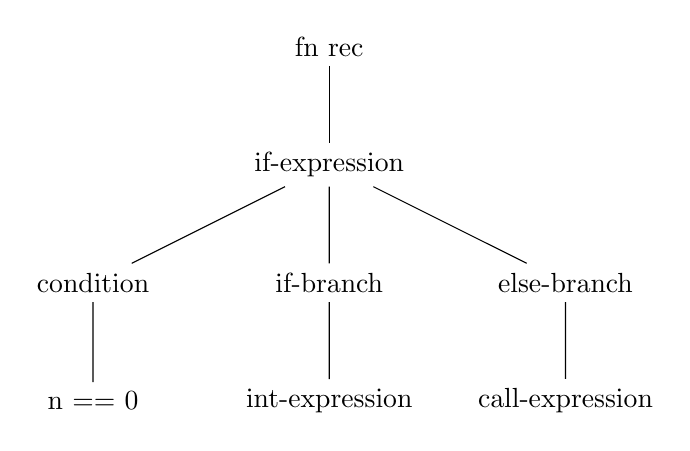
\begin{tikzpicture}[
				tlabel/.style={pos=0.4,right=-1pt,font=\footnotesize\color{red!70!black}},
			]
			\node{fn rec}
			child { node {if-expression}
					child { node {condition} child {node {n == 0}} }
					child [missing]
					child { node {if-branch} child {node {int-expression}} }
					child [missing]
					child { node {else-branch} child{node{call-expression}} }
				};
		\end{tikzpicture}
	\end{adjustbox}
	\caption{Abstract syntax tree and VM instructions of a recursive rush program.}\label{fig:tree_vs_vm_tree}
\end{wrapfigure}

As a conclusion, a VM is often a reasonable approach if an interpreted programming language is to be implemented.
The main advantages of a VM are increased speed, reduced memory usage at runtime, and less runtime errors due to type-checking performed by its compiler.
The main downsides include the need for a compiler targeting the VM, thus making its implementation more demanding compared to a tree-walking interpreter.
Furthermore, debugging the VM is often significantly more demanding than debugging a tree-walking interpreter.
In the past, commercial software has shown that implementing a programming language to run on a virtual machine can indeed be used successfully and on a larger scale.
For instance, the \emph{Java Virtual Machine} (\emph{JMV}) is the software component responsible for executing the compiled \emph{Java bytecode}.
Through the JVM, the compiled Java program preserves its platform independence while using the benefits introduced by a VM~\cite[Chapter~1.2]{Lindholm2014-jb}. %TODO: is chapter the right noun (use section?)
